\documentclass[12pt]{article}

\usepackage[spanish]{babel} % Remove this line if you want English language support
\usepackage[hyperindex]{hyperref}
\usepackage{graphicx}
\usepackage{enumitem}
\usepackage{subfiles} % Best loaded last in the preamble

\addto\captionsspanish{\renewcommand{\contentsname}{Tabla de Contenidos}}

\begin{document}

\title{\textbf{FIUBAKKA} \\ \large \textbf{Juego multijugador online con Akka}}
\author{
    Rolando, Marcos
    \and
    Soriano, Iván
    \and
    Raveszani, Nicole
    \and
    Scaccheri Cassanello, Franco
    \and
    Deymonnaz, Pablo
}
\date{\today}

\maketitle % Prints the title, author, and date

\thispagestyle{empty}

\begin{figure}[htbp]
    \centering
    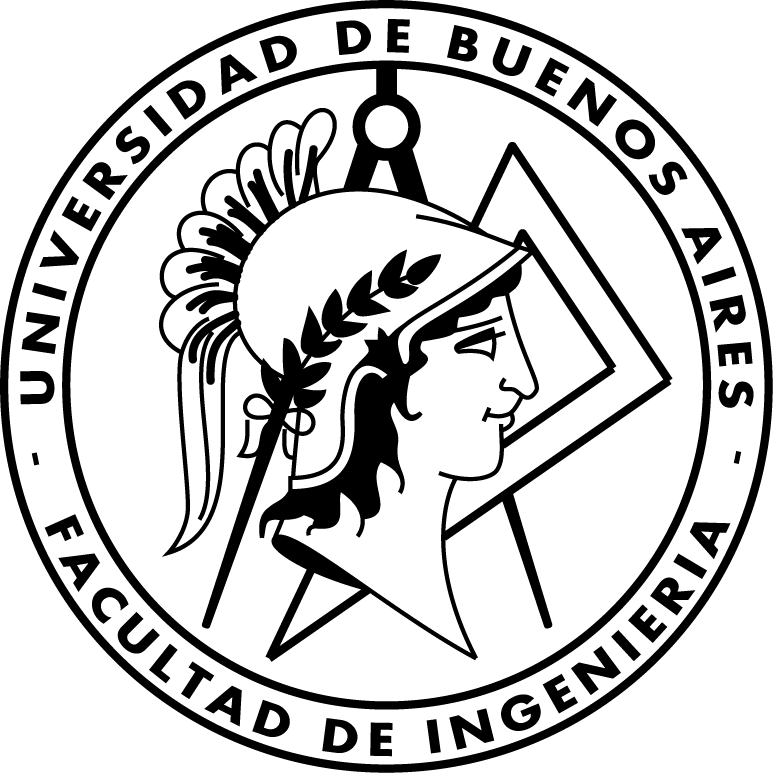
\includegraphics[width=0.5\textwidth]{../assets/fiuba-logo.png}
\end{figure}
\begin{figure}[htbp]
    \centering
    
\includegraphics[width=0.5\textwidth]{../assets/akka-toolkit-logo.png}
\end{figure}

\newpage
\thispagestyle{empty}
\tableofcontents
\newpage

\setcounter{page}{1} % Reset page counter to 1

\section{Resumen / Abstract}

\subfile{resumen.tex}

\vspace{5mm} %5mm vertical space

\subfile{abstract.tex}

\newpage

\section{Introducción}

\subfile{introduction.tex}

\section{Backend: servidor distribuido Akka}
\index{Desarrollo}

\subsection{Introducción a Akka}

\subsection{Arquitectura}

\subsection{Diagramas}

\subsection{Mensajes de Kafka}


\section{Frontend: cliente Godot}

\subsection{Introducción a Godot}

Godot es un motor para desarrollar videojuegos, argentino, gratuito y de código abierto. Este motor permite crear tanto juegos 2D como también juegos 3D. Además de permitir desarrollar para múltiples plataformas, permite programar scripts exponiendo una API orientada a objetos en los lenguajes C++, C\# e incluso GDScript, un lenguaje propio de Godot.

La filosofía del diseño de Godot es construir escenas reutilizables usando nodos. A estas escenas y nodos se les puede agregar comportamiento con scripts. Con la composición y jerarquía de los Nodos, se puede construir una lógica de juego que es clara de entender.

\subsection{Estructura de proyecto}

Para este proyecto, definimos una Escena \textbf{Main} donde instanciamos las escenas del juego necesarias a medida que sean requeridas. Por ejemplo, los niveles propiamente dichos no se instancian al iniciar el juego, sino después de que el jugador se haya conectado al servidor. De esta forma, encapsulamos todas las escenas activas en un mismo lugar y no desperdiciamos recursos instanciando todas las escenas a la vez.

Además hacemos uso de los \textbf{Autoloads} de Godot, que funcionan igual que el patrón \textbf{Singleton}, para ciertas Escenas o scripts que son necesarios en un scope global. Por ejemplo, para el manejo, carga y borrado de escenas, hacemos uso de un \textbf{SceneManager}, que es un script Autoload que permite transicionar entre niveles dentro del juego. 

\subsection{Comunicación con el servidor}

Al comienzo del proyecto, un posible limitante de usar Godot eran las herramientas que podía ofrecer el motor para la conectividad con el servidor, ya sea UDP, TCP o incluso HTTP. Para nuestro beneficio, Godot provee clases y funciones para la comunicación utilizando cualquiera de los protocolos mencionados. En nuestro caso, decidimos usar el protocolo TCP por sus beneficios: conexión mantenida con el servidor, garantía de que se envíen todos los paquetes, etc.

Luego, definimos nuestras propias clases \textit{wrapper} para establecer la conexión al servidor y el manejo de mensajes, tanto para recibirlos (\textbf{ServerConsumer}) como para enviarlos (\textbf{ServerProducer}).

\subsection{Dificultades}

\section{Comunicación entre cliente y servidor}

\subsection{Protocol buffers}

\begin{figure}[htbp]
    \centering
    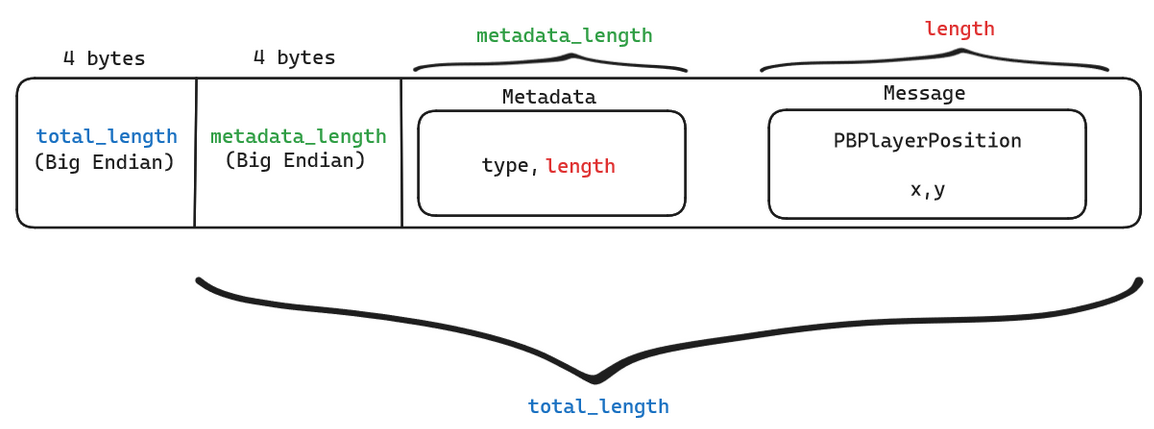
\includegraphics[width=1.0\textwidth]{../assets/protobuf.png}
\end{figure}

\section{Resultados}

\subsection{Resultados esperados}

\subsection{Resultados obtenidos}

\subsection{Métricas de latencia}

\section{Conclusiones}



\end{document}
